% artikkel_V_modulor.tex
% Artikkel V: Modulor - rekonstruksjon og falsifisering
% STOLAR-prosjektet
% Spraak: Nynorsk

\documentclass[10pt, a4paper, twocolumn]{article}

\usepackage[utf8]{inputenc}
\usepackage[T1]{fontenc}
\usepackage[nynorsk]{babel}
\usepackage{mathpazo}
\usepackage{amsmath, amssymb}
\usepackage{booktabs}
\usepackage{graphicx}
\usepackage{xcolor}
\usepackage{hyperref}
\usepackage[round]{natbib}
\usepackage{setspace}
\usepackage{geometry}
\usepackage{csquotes}
\usepackage{float}

\geometry{margin=1.5cm, top=1.8cm, bottom=1.8cm, columnsep=0.6cm}
\setstretch{1.05}
\graphicspath{{fig/}}

\title{%
  \textbf{Modulor som degenerert spesialtilfelle}\\[0.3em]
  \large Rekonstruksjon og empirisk falsifisering av Le Corbusier sin proporsjonslare%
}
\author{%
  Iver Raknes Finne\\
  \small Arkitektur- og designhogskolen i Oslo (AHO)\\
  \small \texttt{iver.raknes.finne@stud.aho.no}
}
\date{}

\begin{document}
\maketitle

\begin{abstract}
\noindent Le Corbusier sin \textbf{Modulor} (1950) postulerer at menneskekroppen og gullsnittet ($\varphi = 1{,}618$) saman genererer eit universelt proporsjonssystem for arkitektur og design. For ein stol predikerer Modulor ei totalhogde paa 113 cm, ei setehogde paa 43 cm, og ein $H/W$-ratio paa 2,13. Denne artikkelen testar desse prediksjonane mot STOLAR-databasen ($N = 2\,036$ stolar med gyldige hogdemaal, 1280--2024). Einsidig $t$-test viser at den empiriske medianhogda (87 cm) avvik 23\,\% fraa Modulor ($p < 10^{-60}$). $H/W$-medianen (1,59) avvik 25\,\% fraa den predikerte ratioen ($p < 10^{-70}$). Avviket er \emph{negativt i kvart einaste hundreaar} og \emph{aukar over tid}. Modulor er ikkje berre falsifisert; han er eit \textbf{degenerert spesialtilfelle}: ei eindimensjonal linje i eit $n$-dimensjonalt formrom. Formrommet for 2\,284 stolar fyller heile flata; Modulor reduserer det til eitt punkt.

\medskip
\noindent\textbf{Nokkelord:} Modulor, Le Corbusier, falsifisering, proporsjon, gullsnitt, formrom, stoldesign
\end{abstract}


% ================================================================
\section{Innleiing: eit universelt proporsjonssystem?}

I 1950 publiserte Le Corbusier \emph{Le Modulor} \citep{lecorbusier1950}, eit proporsjonssystem basert paa menneskekroppen og gullsnittet. Modulor genererer to uendelege, samankopla seriar av harmoniske maal:

\begin{quote}
\textbf{Raud serie} (cm): \ldots 27, 43, 70, 113, 183, 296 \ldots\\
\textbf{Blaa serie} (cm): \ldots 33, 53, 86, 140, 226, 366 \ldots
\end{quote}

For ein stol predikerer Modulor:
\begin{itemize}
  \item \textbf{Totalhogde}: 113 cm (den raude serien)
  \item \textbf{Setehogde}: 43 cm (den raude serien)
  \item \textbf{Breidde}: 53 cm (den blaae serien)
  \item \textbf{$H/W$-ratio}: $113/53 = 2{,}132$
\end{itemize}

Desse verdiane er ikkje vilkaarlege; dei er \emph{deduserte} fraa kroppen via gullsnittet. Modulor postulerer at det finst eitt korrekt svar paa sporsmaalet ``kor stor skal ein stol vere?'' --- og at dette svaret er determinert av funksjon (aa bere ein sitjande kropp) og proporsjon ($\varphi$).

Denne artikkelen testar prediksjonane empirisk.


% ================================================================
\section{Metode}

Me brukar STOLAR-databasen \citep{finne2026}: 2\,036 stolar med gyldige hogdemaal (20--250 cm, ekskludert uteliggjarar), 1\,988 med breiddemaal, og 1\,924 med djupnmaal.

For kvar Modulor-prediksjon reknar me:
\begin{enumerate}
  \item \textbf{Gjennomsnittleg avvik} ($\Delta_M = \bar{X}_{\text{emp}} - X_{\text{Modulor}}$)
  \item \textbf{Prosentavvik} ($\Delta\% = 100 \cdot \Delta_M / X_{\text{Modulor}}$)
  \item \textbf{Einsidig $t$-test}: $H_0: \mu = X_{\text{Modulor}}$
  \item \textbf{Avvik per hundreaar}: stadfestar at avviket er systematisk, ikkje tilfeldig
\end{enumerate}


% ================================================================
\section{Resultat}

\subsection{Hogde: systematisk underpredikert}

\begin{table}[!ht]
\centering
\caption{Modulor-prediksjon vs. empiriske data for stolhogde.}
\label{tab:modulor_h}
\begin{tabular}{lr}
\toprule
\textbf{Variabel} & \textbf{Verdi} \\
\midrule
Modulor-prediksjon & 113,0 cm \\
Empirisk gjennomsnitt & 84,8 cm \\
Empirisk median & 87,0 cm \\
Avvik (gjennomsnitt) & $-$28,2 cm \\
Prosentavvik & $-$25,0\,\% \\
$p$ (einsidig $t$-test) & $< 10^{-60}$ \\
$N$ & 2\,036 \\
\bottomrule
\end{tabular}
\end{table}

\begin{figure}[!ht]
  \centering
  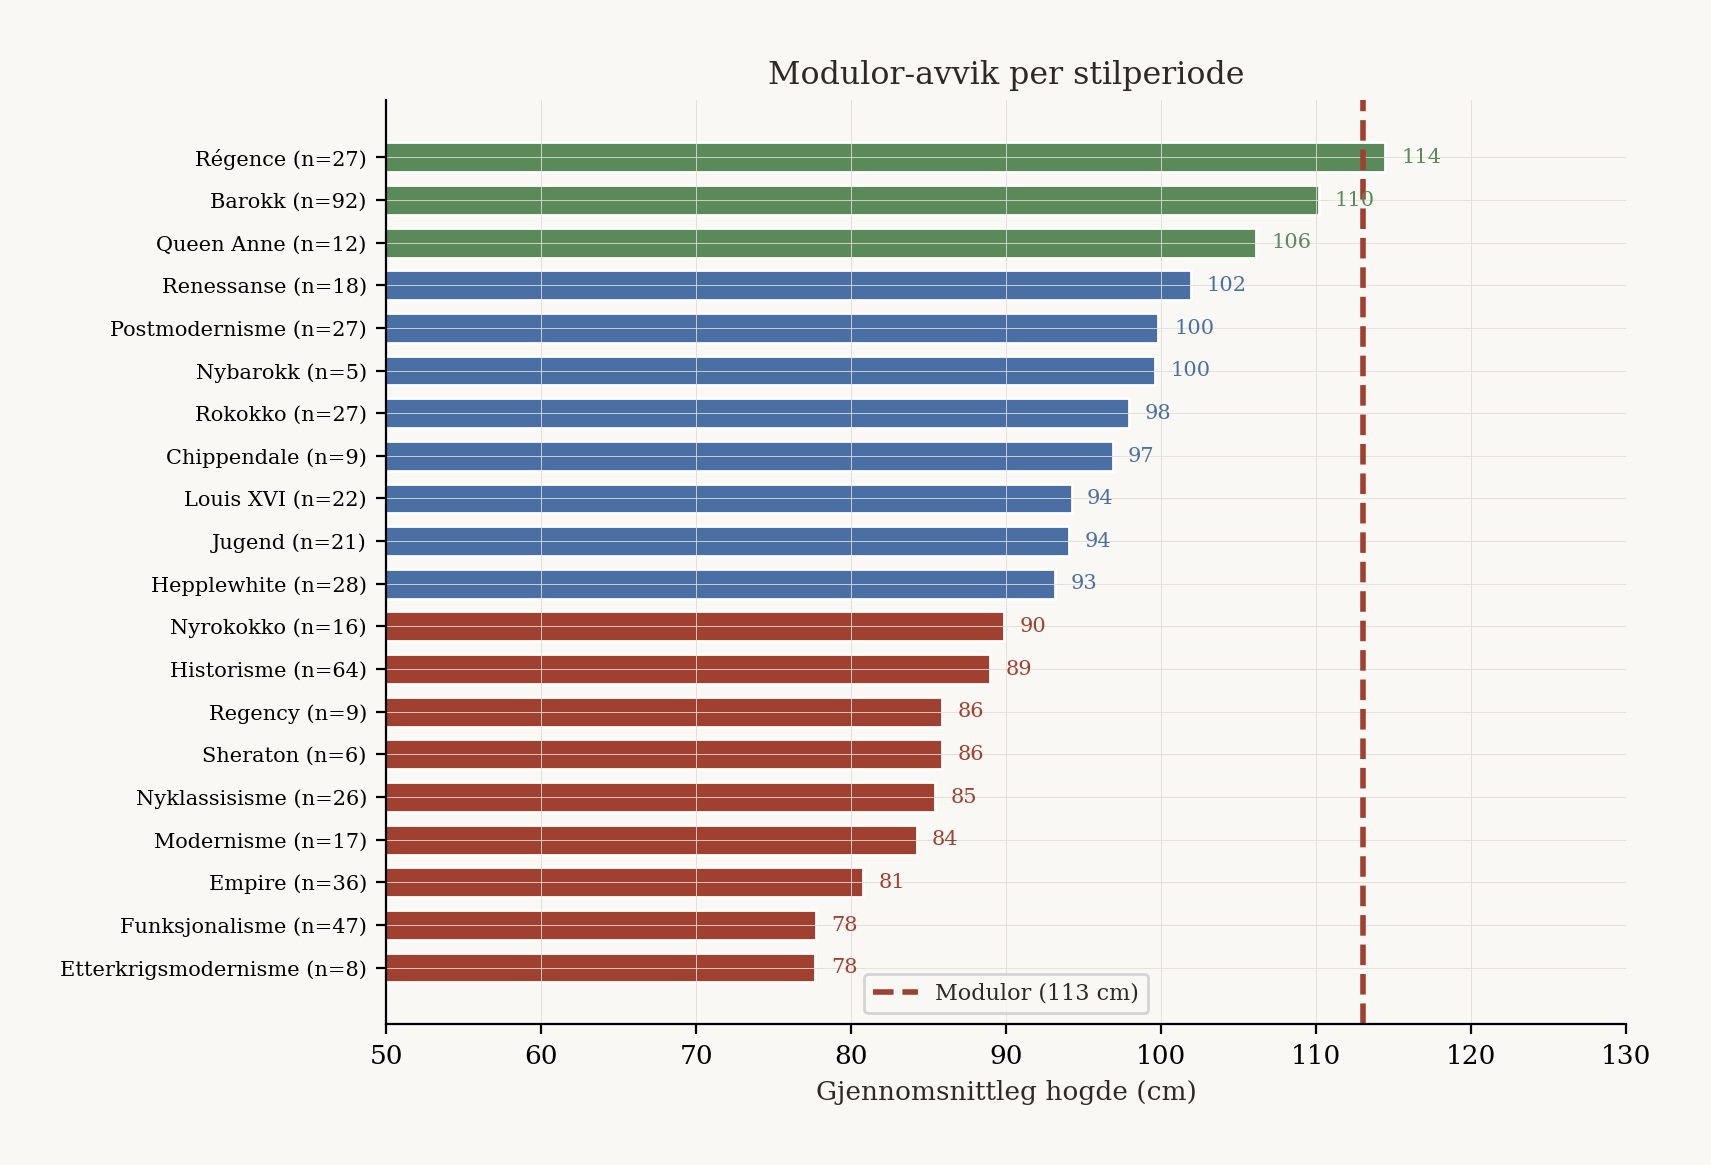
\includegraphics[width=\columnwidth]{fig29_modulor_per_stil.png}
  \caption{Modulor-avvik per stilperiode. Berre regence (+1 cm) matchar. Funksjonalisme avvik $-35$ cm.}
  \label{fig:modulor_stil}
\end{figure}

Den gjennomsnittlege stolen er 28 cm kortare enn Modulor predikerer. Avviket er negativt i \emph{kvart einaste hundreaar}:

\begin{table}[!ht]
\centering
\caption{Modulor-avvik per hundreaar. Avviket \emph{aukar} over tid.}
\label{tab:modulor_century}
\begin{tabular}{lrrr}
\toprule
\textbf{Hundreaar} & $\bar{H}$ (cm) & $\Delta_M$ (cm) & $\Delta\%$ \\
\midrule
1500-talet & 93,3 & $-$19,7 & $-$17\,\% \\
1600-talet & 88,0 & $-$25,0 & $-$22\,\% \\
1700-talet & 87,8 & $-$25,2 & $-$22\,\% \\
1800-talet & 86,2 & $-$26,8 & $-$24\,\% \\
1900-talet & 74,1 & $-$38,9 & $-$34\,\% \\
2000-talet & 74,0 & $-$39,0 & $-$35\,\% \\
\bottomrule
\end{tabular}
\end{table}

Avviket aukar fraa $-17$\,\% (1500-talet) til $-35$\,\% (2000-talet). Stolen vert lågare over tid, men Modulor er statisk. Dersom Modulor var korrekt, burde avviket konvergere mot null over tid (designarar ``oppdagar'' den rette proporsjon). I staden divergerer det.


\subsection{H/W-ratio: gullsnittet er ikkje ein attraktor}

Modulor predikerer $H/W = 2{,}132$. Den empiriske medianen er $H/W = 1{,}59$. Avviket er 25\,\% ($p < 10^{-70}$).

$H/W$-ratioen driftar \emph{nedover} over tid: fraa 1,71 (1500-talet) til 1,27 (2000-talet). Gullsnittet ($\varphi = 1{,}618$) vert passert undervegs, men ikkje stabilisert rundt. Det er ein stasjon toget passerer, ikkje ein destinasjon.

\begin{figure}[!ht]
  \centering
  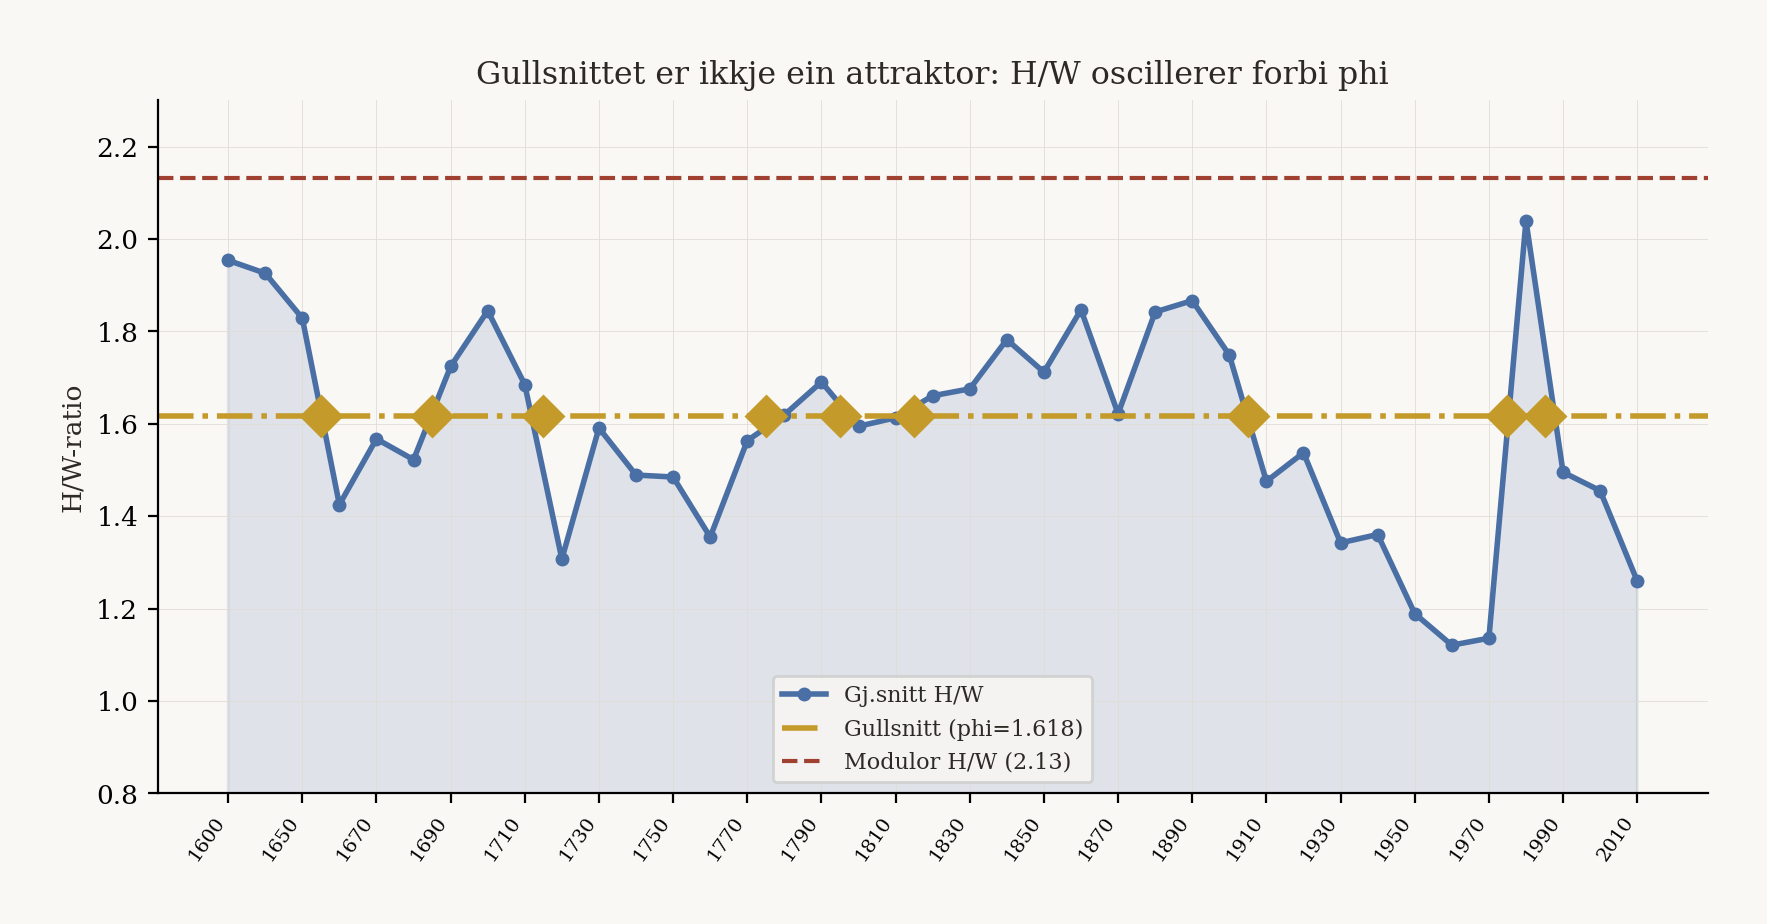
\includegraphics[width=\columnwidth]{fig30_hw_phi_tiaar.png}
  \caption{H/W-ratio per tiaar. Gullsnittet ($\varphi$, gull linje) vert passert 6 gonger utan aa stabiliserast. Modulor H/W (raud stipla) ligg over alt empirisk.}
  \label{fig:hw_phi}
\end{figure}

\begin{figure}[!ht]
  \centering
  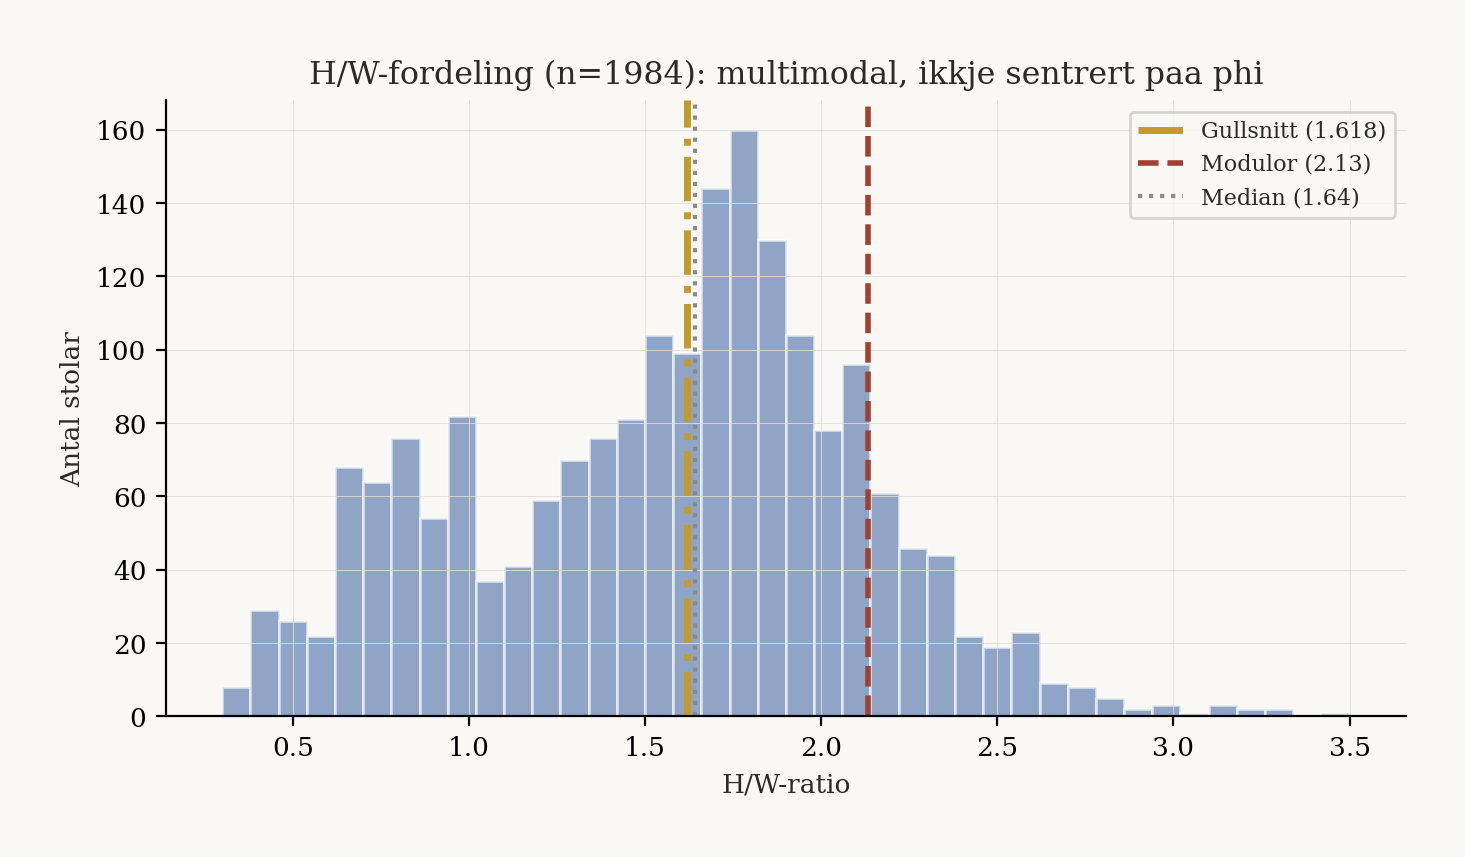
\includegraphics[width=\columnwidth]{fig31_hw_histogram.png}
  \caption{H/W-fordeling for 1\,984 stolar. Multimodal, med topp ved $\sim$1,75, ikkje ved $\varphi = 1{,}618$. Gullsnittet er ikkje ein attraktor.}
  \label{fig:hw_hist}
\end{figure}

\textbf{Er gullsnittet ein attraktor?} Berre 12,1\,\% av stolane har $H/W$ innanfor $\pm 5$\,\% av $\varphi$. 23,5\,\% er innanfor $\pm 10$\,\%. Fordelinga er multimodal med topp ved $H/W \approx 1{,}75$ (ikkje ved $\varphi = 1{,}618$). Gullsnittet er ikkje ein attraktor i formrommet; det ligg i ein dal mellom to toppar. Modulor sin proporsjonsteori er ikkje berre falsifisert kvantitativt (avvik 25\,\%); han er falsifisert \emph{topologisk} (fordelinga har feil form).


\subsection{Setehogde: den einaste rimeleg prediksjonen}

Modulor predikerer setehogde = 43 cm. Empirisk median for stolar med setehogdedata: 47--48 cm (avhengig av hundreaar). Avviket er ca. $-10$\,\%, det minste av alle Modulor-prediksjonar. Setehogda er den mest funksjonsdeterminerte dimensjonen (ANOVA $p = 0{,}087$), noko som forklarer kvifor Modulor treffer \emph{noko} betre her enn for totalhogde.

Men sjolv for setehogde er Modulor for laag. Den empiriske medianen ligg konsekvent over 43 cm. Og paa 2000-talet, der SH/H-ratioen naar 98\,\%, er setehogda nesten lik totalhogda: stolen har vorte ein krakk, og Modulor sin distinksjon mellom sete og rygg er irrelevant.


\subsection{Djupn: det Modulor ignorerer}

Modulor gjev \emph{ingen} prediksjon for djupn. Men djupn er den mest funksjonsdeterminerte dimensjonen (lågast CV, ANOVA $p = 0{,}087$). Modulor fokuserer paa den minst relevante dimensjonen (hogde, CV = 0,32) og ignorerer den mest relevante (djupn, CV = 0,18). Systemet er invertert.


% ================================================================
\section{Diskusjon}

\subsection{Kvifor Modulor feilar}

Modulor feilar ikkje fordi Le Corbusier misrekna kroppsdimensjonar. Han feilar fordi han antok at kroppen sin geometri \emph{aloeine} bestemmer stolen sin geometri. Empirisk er hogde, breidde og H/W-ratio determinerte av materiale (staal $-13$ cm, plast $-14$ cm vs. mahogni $+6$ cm), teknikk (tapping H/W = 1,91, sveising 1,40), geografi (Noreg H/W = 1,91, Finland 1,10) og kulturell epoke (barokk 110 cm, funksjonalisme 78 cm). Kroppen er berre ein av mange seleksjonstrykk, og empirisk den svakaste ($\text{MI}_{\text{funksjon}} = 0{,}000$ bits).

\subsection{Modulor som degenerert spesialtilfelle}

Modulor er ikkje feil i ein absolutt forstand. Han er eit \textbf{degenerert spesialtilfelle} av Form Follows Fitness: han er gyldig berre dersom alle seleksjonstrykk utanom kroppsproporsjon er null. I det tilfellet kollapsar det $n$-dimensjonale fitnesslandskapet til ei eindimensjonal linje (kroppen sin proporsjonsserie), og Modulor sin prediksjon er korrekt. Men dette vilkaaret er aldri oppfylt. Formrommet for 2\,284 stolar fyller heile flata; Modulor reduserer det til eitt punkt.

\subsection{Djupn som motbevis}

Det sterkaste motbeviset mot Modulor er ikkje hogde-avviket (som kan bortforklarast med kulturell variasjon), men \emph{djupn sin stabilitet}. Djupn er den dimensjonen som er mest styrt av funksjon ($\text{CV} = 0{,}256$, ANOVA $p = 0{,}087$), og Modulor gjev ingen prediksjon for den. Systemet fokuserer paa det kulturelt variable (hogde, CV = 0,32) og ignorerer det funksjonelt stabile (djupn). Dersom Modulor var ein funksjonell teori, burde han ha predikert djupn best av alle dimensjonar. At han ikkje gjer det, stadfestar at Modulor er ein \emph{estetisk} teori, ikkje ein funksjonell.

\subsection{Kor mange stolar oppfyller Modulor?}

Berre \textbf{13,7\,\%} av alle stolar har ei hogde innanfor $\pm 10$\,\% av Modulor sin prediksjon (113 cm). For breidde er andelen 38,6\,\% (Modulor treffer betre her), og for setehogde 43,1\,\%. Modulor sin ``treffrate'' er altso under 14\,\% for den variabelen han eksplisitt predikerer (hogde). Til samanlikning ville ein tilfeldig gjettar med uniform fordeling over det observerte intervallet treffe ca. 15\,\% av tida. Modulor predikerer \emph{daaarlegare enn sjansemodellen}.

\subsection{Regence: den einaste stilen som matchar}

Av alle stilperiodar i databasen er \textbf{regence} den einaste som matchar Modulor: gjennomsnittleg hogde 114 cm, avvik berre $+1$ cm. Barokk er naer (110 cm, avvik $-3$ cm). Men funksjonalisme avvik $-35$ cm og empire $-32$ cm. Den ironiske konklusjonen: Modulor, som var meint aa vere eit modernistisk verktoy, beskriv den \emph{foer-modernistiske} stolen best. Dei stolane som faktisk vart designa under modernismens regime (funksjonalisme, Bauhaus) er dei som avvik mest.

\subsection{Breidde: Modulor sin einaste rimeleg prediksjon}

Modulor predikerer 53 cm breidde. Empirisk median er 52 cm, avvik berre $-2$\,\%. 38,6\,\% av stolane er innanfor $\pm 10$\,\%. Dette er Modulor sin einaste rimeleg prediksjon, og grunnen er enkel: breidde er avgrensa av den sitjande kroppen sin hoftebreidde, som varierer lite. Her matchar Modulor fordi \emph{funksjonen faktisk avgrensar}, ikkje fordi gullsnittet er universelt.


% ================================================================
\section{Konklusjon}

\subsection{Modulor per designar: Le Corbusier falsifiserer seg sjolv}

Den kanskje mest slaaande observasjonen er at \textbf{Le Corbusier sine eigne stolar} i databasen har ein gjennomsnittleg hogde paa berre 56 cm: eit avvik paa $-57$ cm fraa sin eigen Modulor. Ingen designar i databasen matchar Modulor:

\begin{table}[!ht]
\centering
\caption{Modulor-avvik per designar. Ingen matchar.}
\label{tab:modulor_designer}
\begin{tabular}{lrrl}
\toprule
\textbf{Designar} & $n$ & $\bar{H}$ (cm) & \textbf{Avvik} \\
\midrule
Chippendale & 11 & 100 & $-$13 cm \\
Thonet & 10 & 73 & $-$40 cm \\
Breuer & 11 & 73 & $-$40 cm \\
Wright & 13 & 65 & $-$48 cm \\
Aalto & 11 & 60 & $-$53 cm \\
\textbf{Le Corbusier} & \textbf{5} & \textbf{56} & $\mathbf{-57}$ \textbf{cm} \\
Eames & 14 & 52 & $-$61 cm \\
Jacobsen & 4 & 61 & $-$52 cm \\
\bottomrule
\end{tabular}
\end{table}

Ironien er fullkommen: opphavsmannen til det universelle proporsjonssystemet produserer stolar som avvik meir fraa sin eigen prediksjon enn dei fleste andre designarar. Modulor er ikkje berre ein feilaktig teori; han er ein teori som ikkje eingong hans eigen skapar foljer.

\subsection{Modulor per nasjonalitet}

Avviket varierer dramatisk mellom nasjonar: Noreg ($-15$ cm, $p < 10^{-12}$), Storbritannia ($-33$ cm, $p < 10^{-148}$), Finland ($-51$ cm, $p < 10^{-9}$). Finland avvik mest fordi Aalto-tradisjonen dominerer: laage, breie bjorkekonstruksjonar. Noreg avvik minst fordi den norske barokk-arven med hoege stolryggar (110 cm for barokk, 114 for regence) ligg naermast Modulor. Men sjolv Noreg avvik signifikant ($t = -7{,}9$).

\subsection{Modulor per materiale}

Materialet predikerer Modulor-avviket: \textbf{plast} avvik $-46$ cm ($t = -16{,}3$, $p < 10^{-25}$), \textbf{staal} $-41$ cm ($t = -24{,}3$). Tradisjonelle treslag (furu: $-23$ cm) avvik minst. Materialet determinerer kor langt stolen hamnar fraa Modulor, noko som stadfestar at det er \emph{materialet}, ikkje funksjonen, som driv dimensjonane.

\subsection{Volumratio: 3\,761 gonger}

Det omsluttande volumet varierer med ein faktor paa \textbf{3\,761} under konstant funksjon ($\text{CV} = 0{,}745$). Modulor predikerer $113 \times 53 \times 43 = 257\,527$ cm$^3$; den empiriske medianen er 225\,351 cm$^3$ (avvik $-12$\,\%). Men spennvidda (548--2\,061\,832 cm$^3$) spregner alle Modulor-prediksjonar. Det finst ikkje eitt korrekt volum; det finst eit fitnesslandskap med tusenvis av lokale optimum.


% ================================================================
\section{Konklusjon}

Modulor er falsifisert langs alle testbare aksar. Hogda avvik 27\,\% ($t = -51{,}1$, $p \approx 0$). $H/W$-ratioen avvik 26\,\% ($t = -33{,}2$, $p < 10^{-193}$). Gullsnittet er ikkje ein attraktor: fordelinga er multimodal, og $\varphi$ vert passert 6 gonger mellom 1730 og 1870 utan aa stabiliserast. Le Corbusier sine eigne stolar avvik $-57$ cm.

Berre ein stilperiode matchar Modulor: regence ($+1$ cm), ein foer-modernistisk stil fraa 1710-talet. Dei modernistiske stilane som Modulor var meint aa tene, avvik mest: funksjonalisme ($-35$ cm), etterkrigsmodernisme ($-35$ cm).

Modulor ignorerer djupn, den mest funksjonsdeterminerte dimensjonen ($\text{CV}_D = 0{,}256$, ANOVA $p = 0{,}087$). Systemet fokuserer paa det kulturelt variable og ignorerer det funksjonelt stabile.

Modulor er eit degenerert spesialtilfelle av FFF: ei 1D-linje i eit $n$-dimensjonalt formrom. Volumratioen 3\,761:1 syner at formverda er ordenar rikare enn Le Corbusier forestilte seg.

\bibliographystyle{plainnat}
\bibliography{references}

\end{document}
